\section{Dataset description}
  The dataset contains eight attributes (or features, denoted by X1...X8) and two responses (or outcomes, denoted by y1 and y2).
  \begin{table}[h!]
  \parbox{.45\linewidth}{
          \centering
          \caption{Features}
          \label{tab:table1}
          \begin{tabular}{|c|}
            Relative compactness (X1)\\
            \hline
            Surface area (X2)\\
            \hline
            Wall area (X3)\\
            \hline
            Roof area (X4)\\
            \hline
            Overall height (X5)\\
            \hline
            Orientation (X6)\\
            \hline
            Glazing area (X7)\\
            \hline
            Glazing area distribution (X8)\\
            \hline            
          \end{tabular}
  }
  \hfill
  \parbox{.45\linewidth}{
          \centering
          \caption{Responses}
          \label{tab:table2}
          \begin{tabular}{|c|}
            Cooling load (y1)\\
            \hline
            Heating load (y2)\\
            \hline           
          \end{tabular}
  }
  \end{table}
  
  \subsection{Mapping}
    The aim is to use the eight features to predict each of the two responses.
    \begin{equation}
         f\colon \begin{array}{>{\displaystyle}r @{} >{{}}c<{{}} @{} >{\displaystyle}l} 
          X &\rightarrow& Y \\ 
          X &\mapsto& f(X) 
         \end{array}
    \end{equation}
        
  \section{Probability density}
  The first step in most data analysis applications is the exploration of the statistical properties of the variables. This is typically achieved   by plotting the probability densities, which succinctly summarize each variable for visualization. One way to obtain an empirical non-parametric density estimate is by using histograms. Although histograms are considered crude for most advanced statistical applications, they have the great advantage of making no prior assumptions regarding the distribution of the examined variable and are very simple to compute. \textit{Often, this preliminary step can reveal whether the variable follows a Gaussian (normal) distribution, which is characterized by a unimodal peak in the middle of the variable’s possible range of values, is completely symmetric}, and is particularly useful because a large number of mathematical functions are applicable \cite{bishop}.

\subsection{Histograms}

\begin{figure}[h!]
    \centering
    \begin{minipage}{0.45\textwidth}
      \centering
      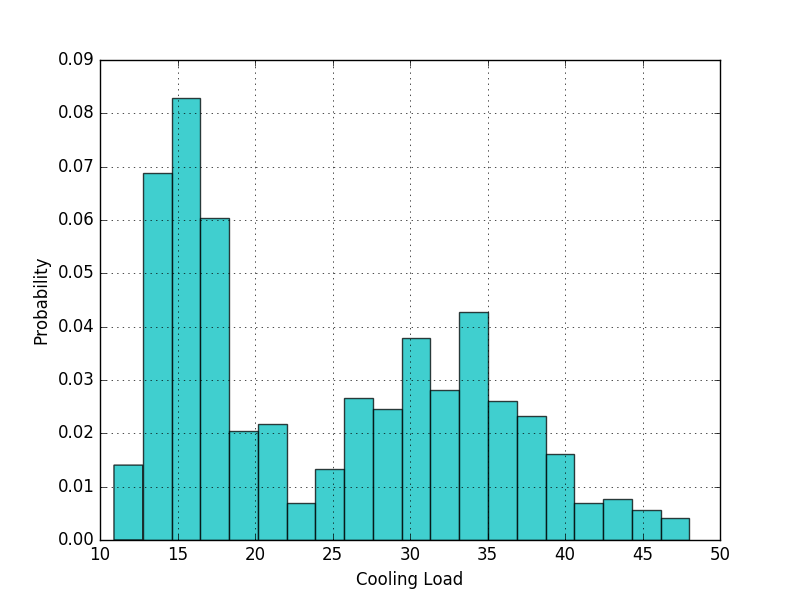
\includegraphics[width=1\textwidth]{hist_cl}
      \caption{Cooling load (y1)}
      \label{fig:hist_cl}
    \end{minipage}\hfill
    \begin{minipage}{0.45\textwidth}
      \centering
      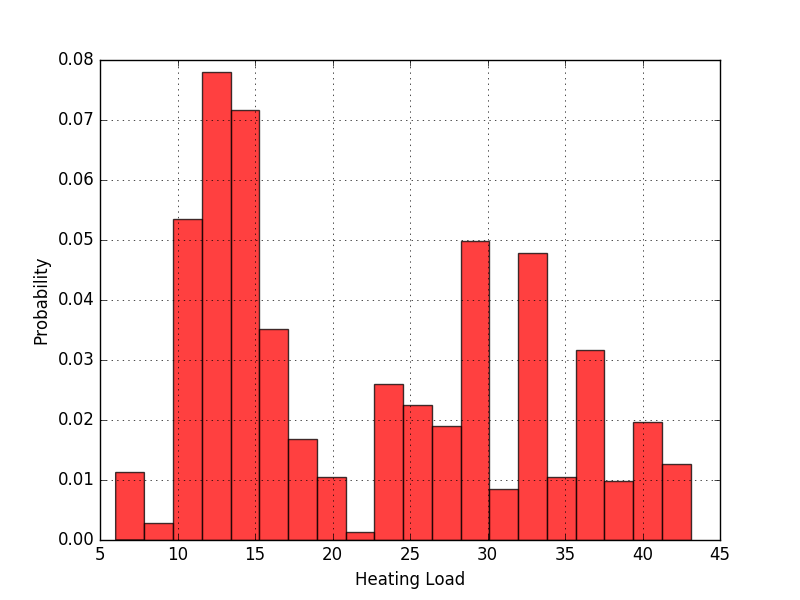
\includegraphics[width=1\textwidth]{hist_hl}
      \caption{Heating load (y2)}
      \label{fig:hist_hl}
    \end{minipage}
\end{figure}
\begin{figure}[h!]
    \centering
    \begin{minipage}{0.45\textwidth}
      \centering
      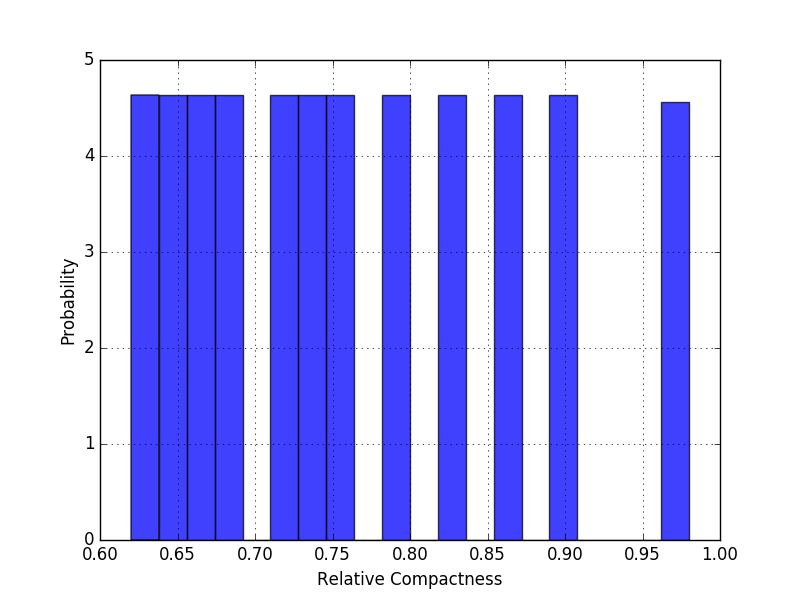
\includegraphics[width=1\textwidth]{hist_rc}
      \caption{Rel. compactness (X1)}
      \label{fig:hist_rc}
    \end{minipage}\hfill
    \begin{minipage}{0.45\textwidth}
      \centering
      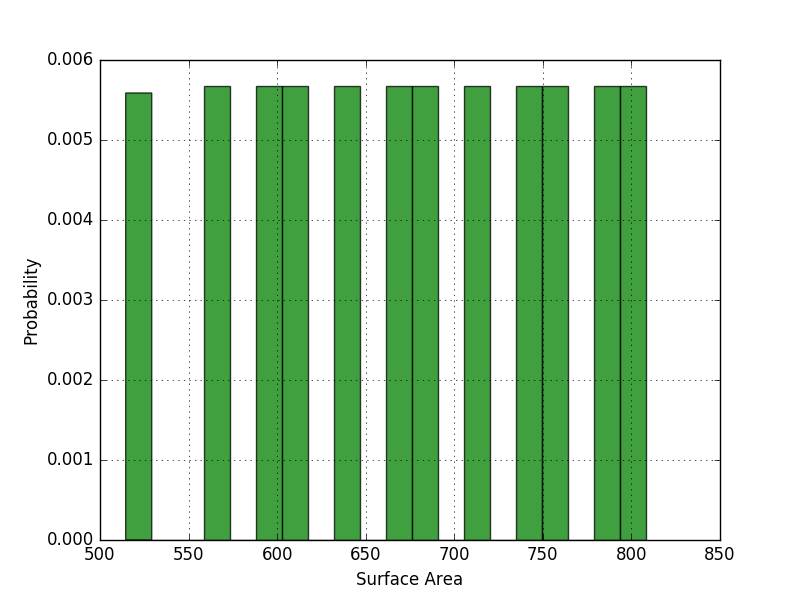
\includegraphics[width=1\textwidth]{hist_sa}
      \caption{Surface area (X2)}
      \label{fig:hist_sa}
    \end{minipage}
\end{figure}
\begin{figure}[h!]
    \centering
    \begin{minipage}{0.45\textwidth}
      \centering
      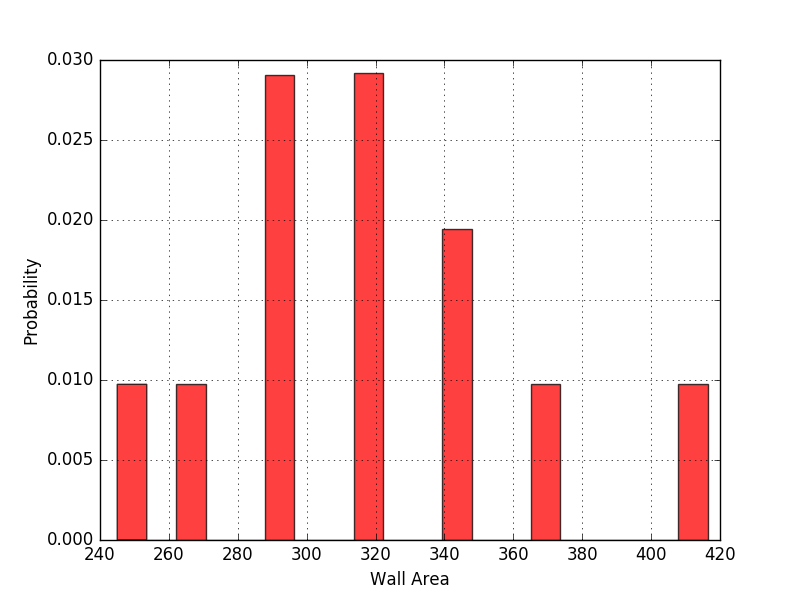
\includegraphics[width=1\textwidth]{hist_wa}
      \caption{Wall area (X3)}
      \label{fig:hist_wa}
    \end{minipage}\hfill
    \begin{minipage}{0.45\textwidth}
      \centering
      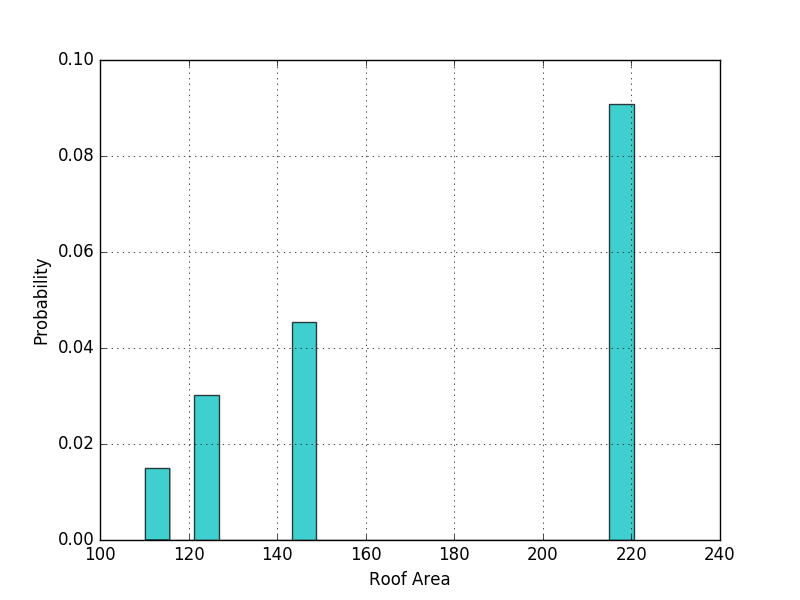
\includegraphics[width=1\textwidth]{hist_ra}
      \caption{Roof area (X4)}
      \label{fig:hist_ra}
    \end{minipage}
\end{figure}
\begin{figure}[h!]
    \centering
    \begin{minipage}{0.45\textwidth}
      \centering
      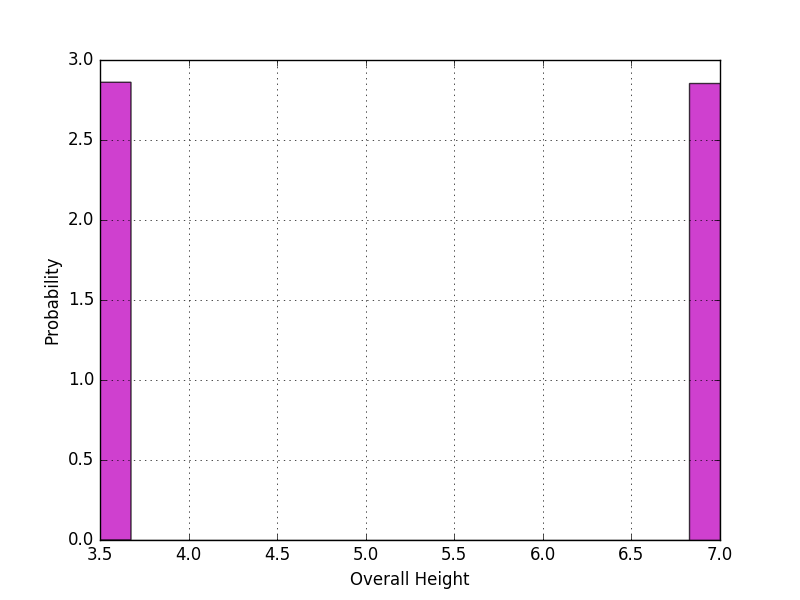
\includegraphics[width=1\textwidth]{hist_oh}
      \caption{Overall height (X5)}
      \label{fig:hist_oh}
    \end{minipage}\hfill
    \begin{minipage}{0.45\textwidth}
      \centering
      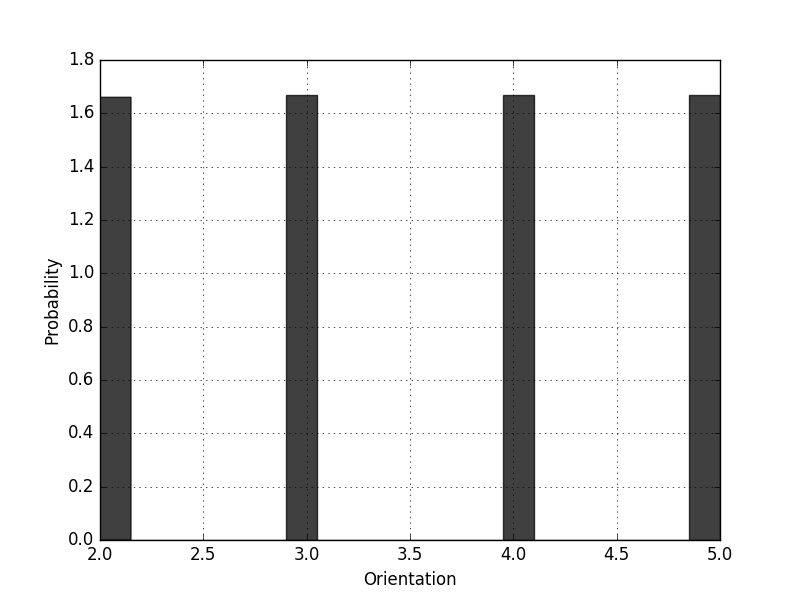
\includegraphics[width=1\textwidth]{hist_or}
      \caption{Orientation (X6)}
      \label{fig:hist_or}
    \end{minipage}
\end{figure}
\begin{figure}[h!]
    \centering
    \begin{minipage}{0.45\textwidth}
      \centering
      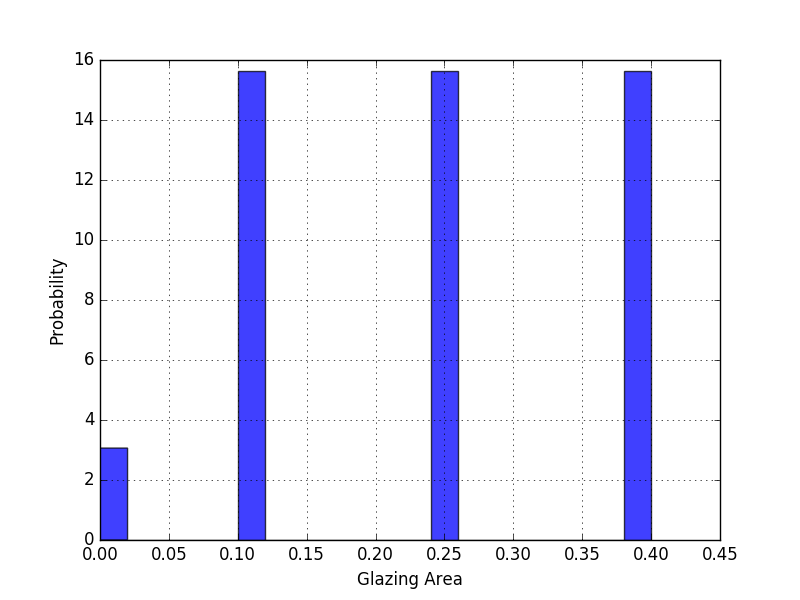
\includegraphics[width=1\textwidth]{hist_ga}
      \caption{Glazing area (X7)}
      \label{fig:hist_ga}
    \end{minipage}\hfill
    \begin{minipage}{0.45\textwidth}
      \centering
      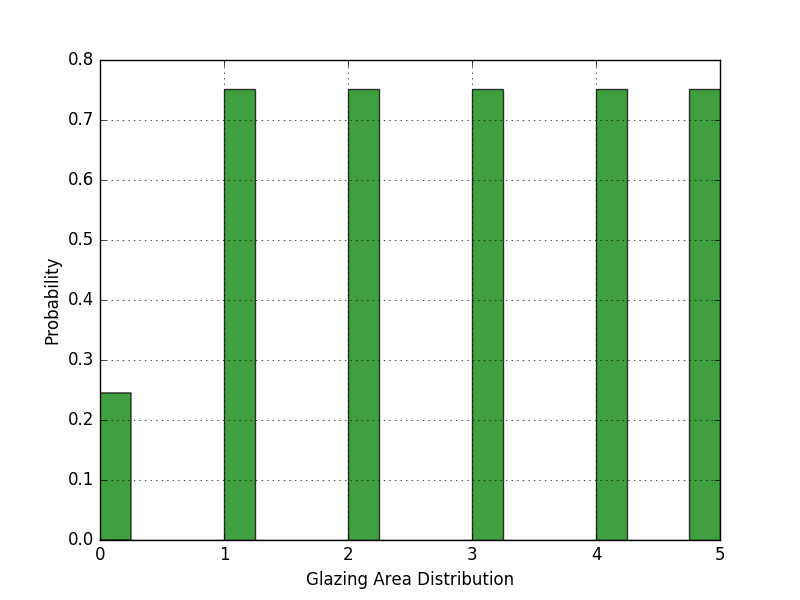
\includegraphics[width=1\textwidth]{hist_gad}
      \caption{Glazing area distribution (X8)}
      \label{fig:hist_gad}
    \end{minipage}
\end{figure}
\newpage
\subsection{Conclusion}
We observe that there is no unimodal peak in the middle or the symmetry. Hence, the data is non-Gaussian.

\section{Correlation}
  \subsection{Scatter plot}
    Scatter plots are similar to line graphs in that they use horizontal and vertical axes to plot data points. However, they have a very specific purpose. Scatter plots show how much one variable is affected by another. The relationship between two variables is called their correlation. For simplicity, scatter plots often use normalized data (i.e. all the variables are normalized to lie between 0 and 1) to facilitate comparison between measures that possibly span orders of magnitude different ranges of values.
Correlation plot between different features and between features and responses have been shown below:    
    \begin{figure}
      \centering
      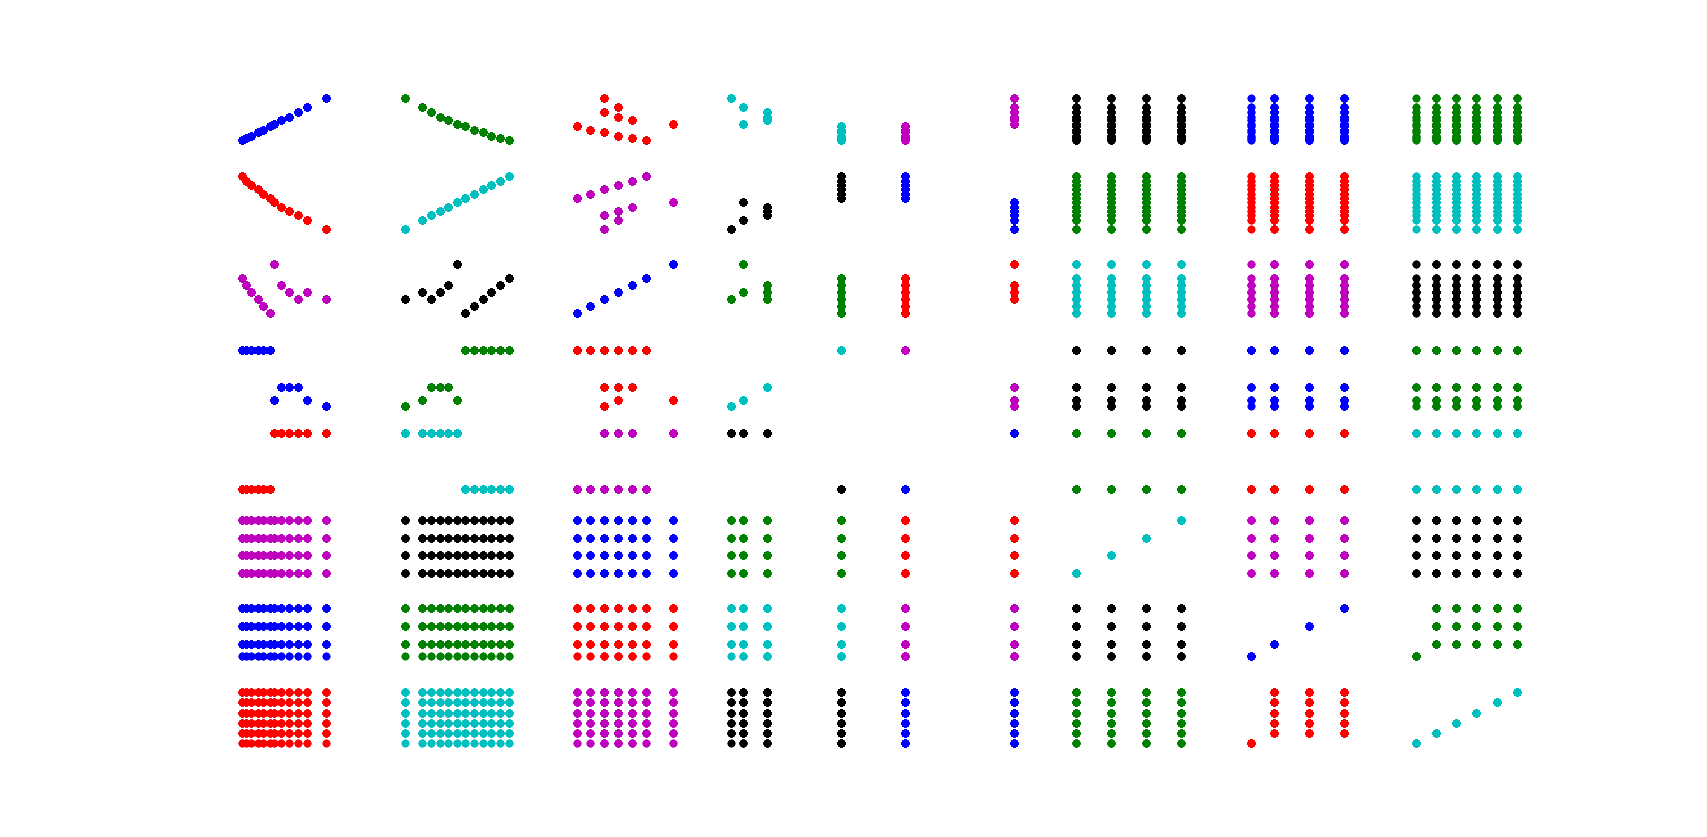
\includegraphics[width=1\textwidth]{scatter_xx}
      \caption{Scatter plot grid between features (X)}
      \label{fig:scatter_xx}
    \end{figure}
    \begin{figure}
      \centering
      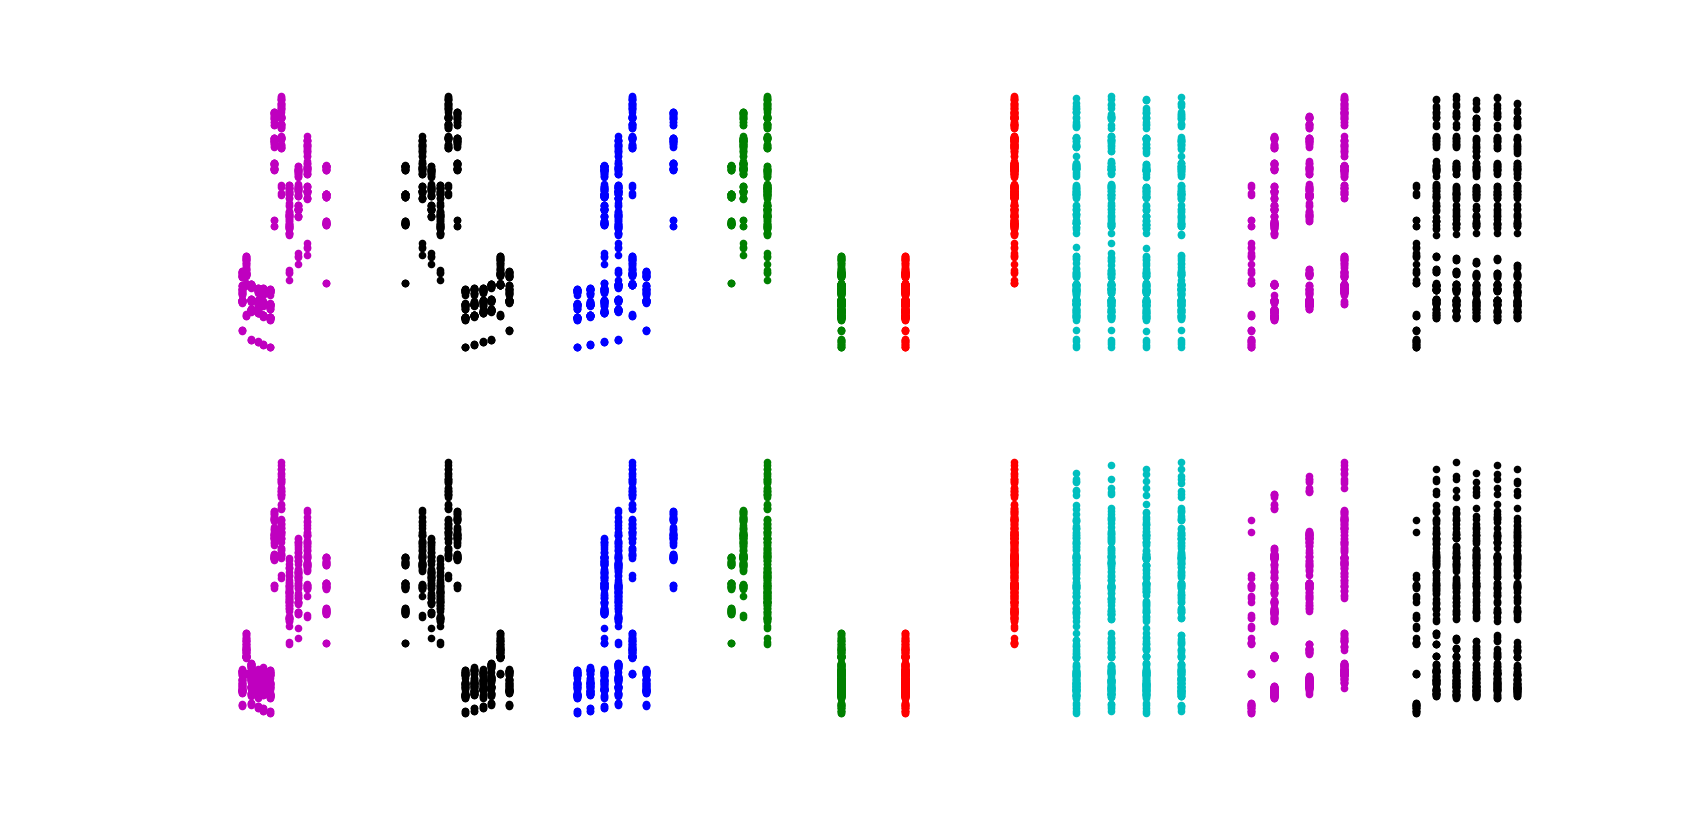
\includegraphics[width=1\textwidth]{scatter_xy}
      \caption{Scatter plot grid between features (X) vs responses (Y)}
      \label{fig:scatter_xy}
    \end{figure}
  \subsection{Spearman rank correlation coefficient}
    As concluded from the histogram plot above, the data is non-Gaussian, so we use the Spearman rank correlation coefficient to obtain a statistical metric regarding the association strength of each input variable with each of the two outputs. The Spearman rank correlation coefficient can characterize general monotonic relationships and lies in the range [-1 1], where negative sign indicates inversely proportional and positive sign indicates proportional rela- tionship, whilst the magnitude denotes how strong this relationship is.
    \begin{figure}[htbp]
      \hspace*{-2.1cm}
      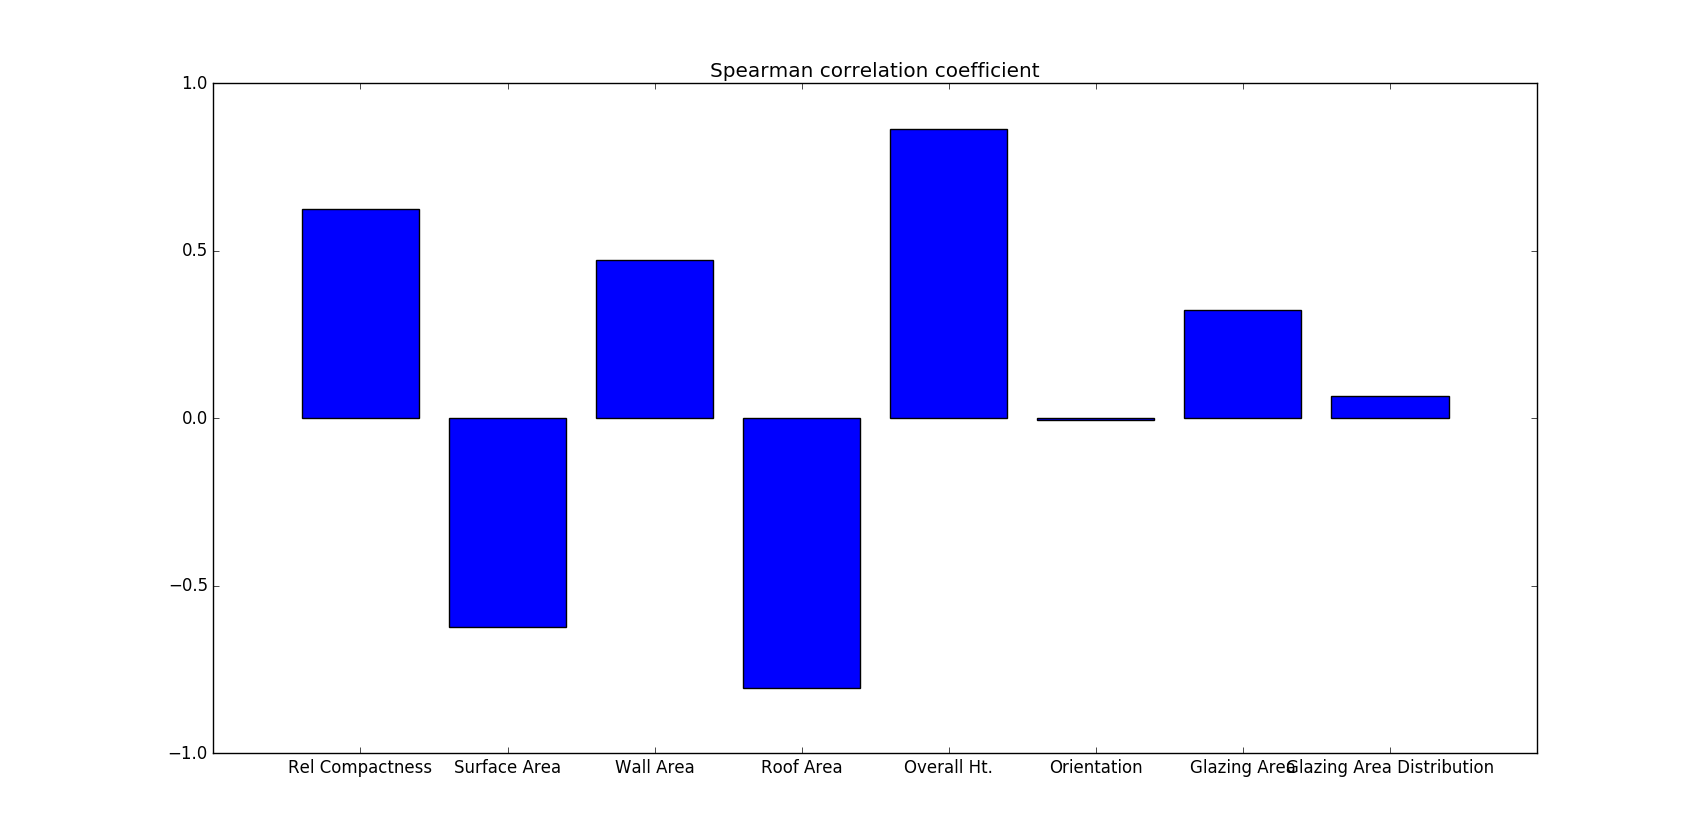
\includegraphics[width=1.3\textwidth]{sp_coeff}
      \caption{Spearman rank correlation coeff. for various features}
      \label{fig:sp_coeff}
    \end{figure}
    \newpage
    \begin{table}[h!]
          \centering
          \caption{Association strength estimated using the Spearman rank correlation coefficient of the eight input variables (X1. . . X8) with heating load (y1).}
          \label{tab:sprcoeffhl}
          \begin{tabular}{c|c}
            Features & Spearman rank correlation coefficient\\
            \hline
            X1 & 0.623 \\
            \hline
            X2 & -0.623 \\
            \hline
            X3 & 0.471 \\
            \hline
            X4 & -0.806 \\
            \hline
            X5 & 0.861 \\
            \hline
            X6 & -0.004 \\
            \hline
            X7 & 0.323 \\
            \hline
            X8 & 0.068 \\
            \hline
          \end{tabular}
    \end{table}
    
    \begin{table}[h!]
          \centering
          \caption{Association strength estimated using the Spearman rank correlation coefficient of the eight input variables (X1. . . X8) with cooling load (y2).}
          \label{tab:sprcoeffcl}
          \begin{tabular}{c|c}
            Features & Spearman rank correlation coefficient\\
            \hline
            X1 & 0.651 \\
            \hline
            X2 & -0.651 \\
            \hline
            X3 & 0.416 \\
            \hline
            X4 & -0.803 \\
            \hline
            X5 & 0.865 \\
            \hline
            X6 & 0.018 \\
            \hline
            X7 & 0.289 \\
            \hline
            X8 & 0.046 \\
            \hline
          \end{tabular}
    \end{table}
    \subsection{Correlation Matrix for features(X)}
          \begin{equation}
            \Corr(X, Y) = \frac{\Cov(X, Y)}{\sigma_{x}\sigma_{y}} = \frac{\E[(X-\mu_{x})(Y-\mu_{y})]}{\sigma_{x}\sigma_{y}}  
          \end{equation}
          \newline
          \begin{equation}
            \left[
              \begin{matrix}
                  1.0 & -1.0 & -0.254 & -0.870 & 0.869 & 0.002 & 0.003 & 0.003\\
-1.0 & 1.0 & 0.254 & 0.870 & -0.869 & -0.002 & -0.004 & -0.003\\
-0.254 & 0.254 & 1.0 & -0.195 & 0.221 & -0.001 & -0.001 & -0.001\\
-0.870 & 0.870 & -0.195 & 1.0 & -0.937 & -0.003 & -0.003 & -0.003\\
0.869 & -0.869 & 0.221 & -0.937 & 1.0 & 0.002 & 0.002 & 0.002\\
0.002 & -0.002 & -0.001 & -0.003 & 0.002 & 1.0 & -0.003 & -0.003\\
0.003 & -0.004 & -0.002 & -0.003 & 0.002 & -0.003 & 1.0 & 0.184\\
0.003 & -0.003 & -0.001 & -0.003 & 0.002 & -0.003 & 0.184 & 1.0
              \end{matrix}
            \right]
    \end{equation}
    \begin{figure}[htbp]
      \hspace*{-6.1cm}
      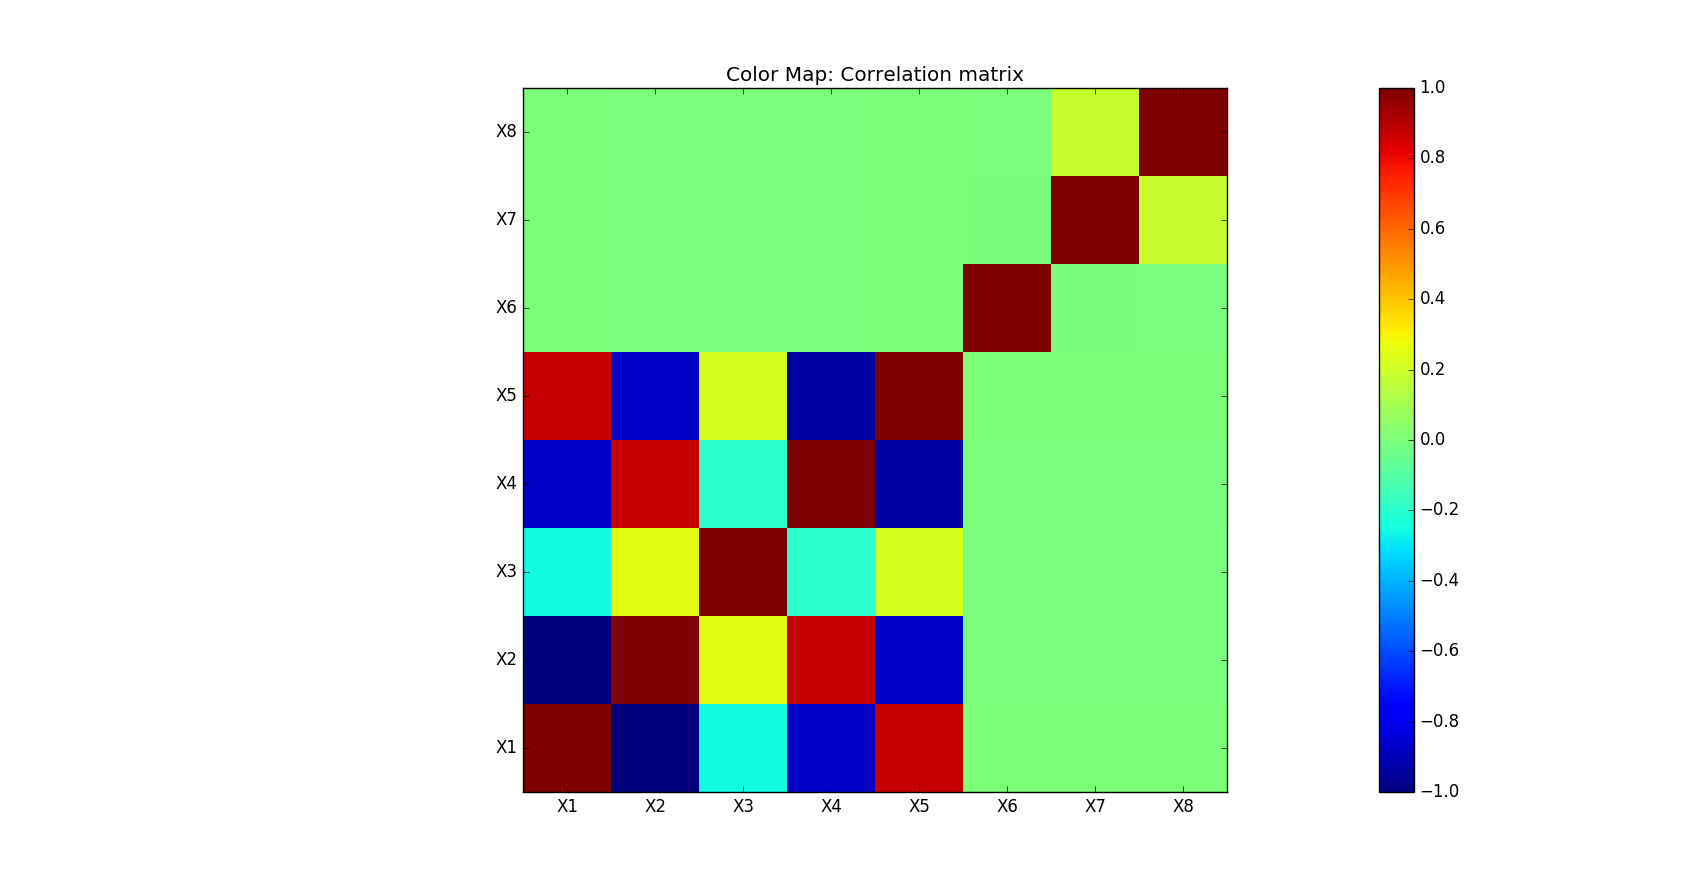
\includegraphics[width=1.7\textwidth]{cov_matrix}
      \caption{Correlation matrix shown as Color Map}
      \label{fig:cov_matrix}
    \end{figure}
    \newpage  
  \subsection{Conclusion}
  Figure \ref{fig:hist_rc} presents the empirical probability distributions of all the input and output variables. These distributions demonstrate that none of the variables follows the normal distribution. Figure \ref{fig:scatter_xy} displays the scatter plots for each of the (normalized) input variables with each of the two output variables. These scatter plots and Color Map show that any functional relationship of the input variables and the output variables is not trivial. This suggests that we can reasonably expect that classical learners such as linear regression (linear models) may fail to find an accurate mapping of the input variables to the output variables. Therefore, these plots intuitively justify the need to experiment with complicated learners such as Artificial Neural Networks (non linear models).
